

\twocolumn[{
	\renewcommand\twocolumn[1][]{#1}
	\begin{center}
		\textbf{\Large Appendix:\\Are Transformers Effective for Time Series Forecasting?}\end{center}
}]

%
In this Appendix, we provide descriptions of non-Transformer-based TSF solutions, detailed experimental settings, more comparisons under different look-back window sizes, and the visualization of \modelname on all datasets. We also append our code to reproduce the results shown in the paper.



\appendix


\section{Related Work: Non-Transformer-Based TSF Solutions}
\label{sec:related_non}
As a long-standing problem with a wide range of applications, statistical approaches (e.g., autoregressive integrated moving average (ARIMA)~\cite{ariyo2014arima}, exponential smoothing~\cite{gardner1985exponential}, and structural models~\cite{harvey1990forecasting}) for time series forecasting have been used from the 1970s onward.
%
Generally speaking, the parametric models used in statistical methods require significant domain expertise to build. 

To relieve this burden, many machine learning techniques such as gradient boosting regression tree (GBRT)~\cite{gbrt,elsayed2021we} 
%and gaussian processes~\cite{roberts2013gaussian} 
gain popularity, which learns the temporal dynamics of time series in a data-driven manner. 
%
However, these methods still require manual feature engineering and model designs.
%
With the powerful representation learning capability of deep neural networks (DNNs) from abundant data, various deep learning-based TSF solutions are proposed in the literature, achieving better forecasting accuracy than traditional techniques in many cases. 

Besides Transformers, the other two popular DNN architectures are also applied for time series forecasting: 

\begin{itemize}
    \item Recurrent neural networks (RNNs) based methods (e.g.,~\cite{petnehazi2019recurrent}) summarize the past information compactly in internal memory states and recursively update themselves for forecasting. 
    \item Convolutional neural networks (CNNs) based methods (e.g.,~\cite{bai2018empirical}), wherein convolutional filters are used to capture local temporal features.
\end{itemize}

RNN-based TSF methods belong to IMS forecasting techniques. Depending on whether the decoder is implemented in an autoregressive manner, there are either IMS or DMS forecasting techniques for CNN-based TSF methods~\cite{bai2018empirical,liu2021time}. 

\section{Experimental Details}
\label{sec:supp_exp}
\subsection{Data Descriptions}
We use nine wildly-used datasets in the main paper. The details are listed in the following.
%
\begin{itemize}
\item ETT (Electricity Transformer Temperature)~\cite{informer}\footnote{\url{https://github.com/zhouhaoyi/ETDataset}} consists of two hourly-level datasets (ETTh) and two 15-minute-level datasets (ETTm). Each of them contains seven oil and load features of electricity transformers from July $2016$ to July $2018$.
%
\item Traffic\footnote{\url{http://pems.dot.ca.gov}} describes the road occupancy rates. It contains the hourly data recorded by the sensors of San Francisco freeways from $2015$ to $2016$. 
%
\item Electricity\footnote{\url{https://archive.ics.uci.edu/ml/datasets/ElectricityLoadDiagrams20112014}} collects the hourly electricity consumption of $321$ clients from $2012$ to $2014$.
%
\item Exchange-Rate~\cite{GuokunLai2017lstm}\footnote{\url{https://github.com/laiguokun/multivariate-time-series-data}} collects the daily exchange rates of $8$ countries from $1990$ to $2016$.
%
\item Weather\footnote{\url{https://www.bgc-jena.mpg.de/wetter/}} includes $21$ indicators of weather, such as air temperature, and humidity. Its data is recorded every 10 min for $2020$ in Germany.
%
\item ILI\footnote{\url{https://gis.cdc.gov/grasp/fluview/fluportaldashboard.html}} describes the ratio of patients seen with influenza-like illness and the number of patients. It includes weekly data from the Centers for Disease Control and Prevention of the United States from $2002$ to $2021$.

\end{itemize}


\subsection{Implementation Details}
% 每个方法使用的来源
For existing Transformer-based TSF solutions: the implementation of Autoformer~\cite{xu2021autoformer}, Informer~\cite{informer}, and the vanilla Transformer~\cite{vaswani2017attention} are all taken from the Autoformer work~\cite{xu2021autoformer}; the implementation of FEDformer~\cite{zhou2022fedformer} and Pyraformer~\cite{liu2021pyraformer} are from their respective code repository. We also adopt their default hyper-parameters to train the models. For \emph{DLinear}, the moving average kernel size for decomposition is 25, which is the same as Autoformer. The total parameters of a vanilla linear model and a \emph{NLinear} are T\*L. The total parameters of the \emph{DLinear} are 2\*T\*L. Since \modelname will be underfitting when the input length is short, and LTSF-Transformers tend to overfit on a long lookback window size. To compare the best performance of existing LTSF-Transformers with \modelname, we report L=336 for \modelname and L=96 for Transformers by default. For more hyper-parameters of \modelname, please refer to our code.



\section{Additional Comparison with Transformers}
\label{sec:supp_add}
We further compare \modelname with LTSF-Transformer for  Univariate Forecasting on four ETT datasets. Moreover, in Figure $4$ of the main paper, we demonstrate that existing Transformers fail to exploit large look-back window sizes with two examples. Here, we give comprehensive comparisons between \modelname and Transformer-based TSF solutions under various look-back window sizes \emph{on all benchmarks}.
%to further validate their ineffectiveness.  



\subsection{Comparison of Univariate Forecasting}

We present the univariate forecasting results on the four ETT datasets in table~\ref{tab:uni-benchmarks-ett}. Similarly, \modelname, especially for \emph{NLinear} can consistently outperform all transformer-based methods by a large margin in most time. We find that there are serious distribution shifts between training and test sets (as shown in Fig.~\ref{fig:distribution_shift} (a), (b)) on ETTh1 and ETTh2 datasets. Simply normalization via the last value from the lookback window can greatly relieve the distribution shift problem.

\begin{table*}[h]
\centering
\scalebox{0.85}{
\begin{tabular}{c|c|cccccc|ccccccccccc}
\hline
\multicolumn{2}{c|}{Methods}&\multicolumn{2}{c|}{Linear}&\multicolumn{2}{c|}{NLinear}&\multicolumn{2}{c|}{DLinear}&\multicolumn{2}{c|}{FEDformer-f}&\multicolumn{2}{c|}{FEDformer-w}&\multicolumn{2}{c|}{Autoformer}&\multicolumn{2}{c|}{Informer}&\multicolumn{2}{c}{LogTrans}\\
\hline
\multicolumn{2}{c|}{Metric} & MSE  & MAE & MSE  & MSE  & MAE & MAE & MSE & MAE& MSE  & MAE& MSE  & MAE& MSE  & MAE& MSE  & MAE\\
\hline

\multirow{4}{*}{\rotatebox{90}{$ETTh1$}}
&96 &0.189	&0.359	&\textbf{0.053}	&\textbf{0.177}	& {0.056} &{0.180} &0.079 &0.215 &0.080 &0.214 &{\underline{0.071}} &{\underline{0.206}}&	0.193&	0.377&	0.283&	0.468\\
&192 &0.078	&0.212	&\textbf{0.069}	&\textbf{0.204}	& {0.071}	&{0.204} &{\underline{0.104}} &{\underline{0.245}} &0.105 &0.256 & 0.114 &	0.262&	0.217&	0.395&	0.234&	0.409\\
&336 &0.091	&0.237	&\textbf{0.081}	&\textbf{0.226}	& {0.098}	&{0.244} &0.119 &0.270 &0.120 &0.269 &{\underline{0.107}}&{\underline{0.258}} &0.202&	0.381&	0.386&	0.546\\
&720 &0.172	&0.340	&\textbf{0.080}	&\textbf{0.226}	&0.189	&0.359 &0.142 &0.299 & {0.127} &{0.280} &{\underline{0.126}}&{\underline{0.283}} &0.183&	0.355&	0.475&	0.629\\
\hline
\multirow{4}{*}{\rotatebox{90}{$ETTh2$}}
&96 &0.133	&0.283	&\textbf{0.129}	&\textbf{0.278}	&0.131	&0.279 &{\underline{0.128}} &{\underline{0.271}} &0.156 &0.306 & 0.153&	0.306&	0.213&	0.373&	0.217&	0.379\\
&192 &0.176	&0.330	&\textbf{0.169}	&\textbf{0.324}	&{0.176}	&{0.329} &{\underline{0.185}} &{\underline{0.330}} &0.238 &0.380 & 0.204&	0.351&	0.227&	0.387&	0.281&	0.429\\
&336 &0.213	&0.371	&\textbf{0.194}	&\textbf{0.355}	&{0.209}	&{0.367} &{\underline{0.231}} &{\underline{0.378}} &0.271 &0.412 & 0.246&	0.389&	0.242&	0.401&	0.293&	0.437\\
&720 &0.292	&0.440	&\textbf{0.225}	&\textbf{0.381}	&0.276	&0.426 &0.278 &{{0.420}} &0.288 &0.438 & {\underline{0.268}}&	{\underline{0.409}}&	0.291&	0.439&	0.218&	0.387\\
\hline
\multirow{4}{*}{\rotatebox{90}{$ETTm1$}}
&96 &0.028	&0.125	&\textbf{0.026}	&\textbf{0.122}	&{0.028}	&{0.123} &{\underline{0.033}} &{\underline{0.140}} &0.036 &0.149 & 0.056&	0.183&	0.109&	0.277&	0.049&	0.171\\
&192 &0.043	&0.154	&\textbf{0.039}	&\textbf{0.149}	&{0.045}	&{0.156} &{\underline{0.058}} &{\underline{0.186}} &0.069 &0.206 & 0.081&	0.216&	0.151&	0.310&	0.157&	0.317\\
&336 &0.059	&0.180	&\textbf{0.052}	&\textbf{0.172}	&{0.061}	&{0.182} &0.084 &0.231 &{\underline{0.071}} &{\underline{0.209}} & 0.076&	0.218&	0.427&	0.591&	0.289&	0.459\\
&720 &0.080	&0.211	&\textbf{0.073}	&\textbf{0.207}	&{0.080}	&{0.210} &{\underline{0.102}} &0.250 &0.105 &{\underline{0.248}} & 0.110&	0.267&	0.438&	0.586&	0.430&	0.579\\
\hline
\multirow{4}{*}{\rotatebox{90}{$ETTm2$}} 
& 96 &0.066	&0.189	&\textbf{0.063}	&\textbf{0.182}	&{0.063}	&{0.183} & 0.067 & 0.198 &{\underline{0.063}} &{\underline{0.189}} & 0.065 & 0.189 & 0.088 & 0.225 & 0.075 & 0.208   \\
& 192 &0.094	&0.230	&\textbf{0.090}	&\textbf{0.223}	&{0.092}	&{0.227} & {\underline{0.102}} & {\underline{0.245} }&0.110 &0.252 & 0.118 & 0.256 & 0.132 &0.283 & 0.129 &0.275     \\
& 336 &0.120	&0.263	&\textbf{0.117}	&\textbf{0.259}	&{0.119}	&{0.261} & {\underline{0.130}} & {\underline{0.279} }&0.147 &0.301 & 0.154 & 0.305  &0.180 &0.336 & 0.154 &0.302      \\
& 720 &0.175	&0.320	&\textbf{0.170}	&\textbf{0.318}	&{0.175}	&{0.320}& {\underline{0.178}} & {\underline{0.325}} &0.219 &0.368 & 0.182 &0.335  &0.300  &0.435 & 0.160 &0.321       \\
\hline
\end{tabular}
}
\caption{Univariate long sequence time-series forecasting results on ETT full benchmark. The \textbf{best results} are highlighted in { \textbf{bold}} and the \underline{best results of Transformers} are highlighted with a { \underline{underline}}.}
\label{tab:uni-benchmarks-ett}
\end{table*}

\begin{figure*}[h]	
	\subfigure[ETTh1 channel6]
	{
		\begin{minipage}{4.1cm}
			\centering     
			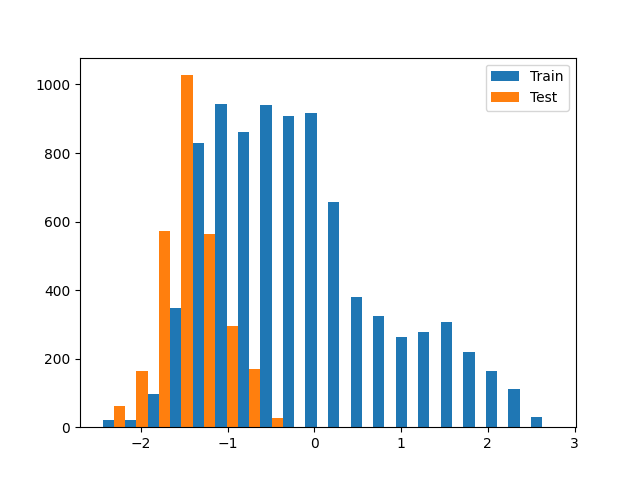
\includegraphics[scale=0.29]{img/ETTh1_channel6.png}
		\end{minipage}
	}
	\subfigure[ETTh2 channel3]
	{
		\begin{minipage}{4.1cm}
			\centering     
			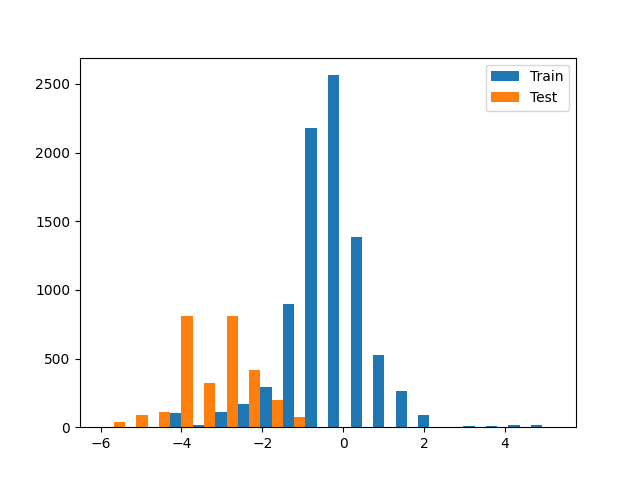
\includegraphics[scale=0.29]{img/ETTh2_channel3.png} 
		\end{minipage}
	}
	\subfigure[Electricity channel3]
	{
		\begin{minipage}{4.1cm}
			\centering     
			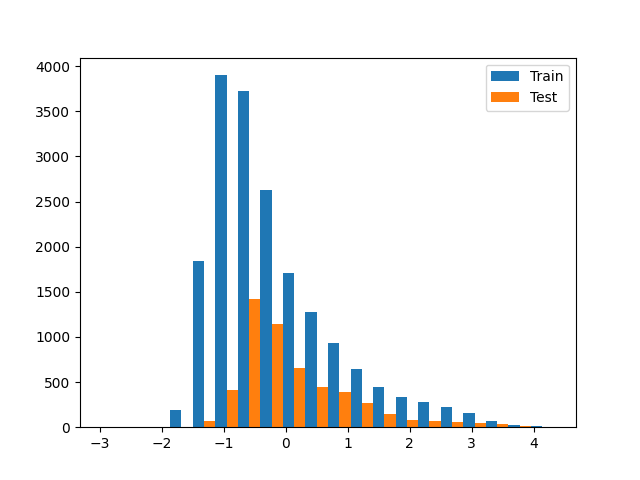
\includegraphics[scale=0.29]{img/ELE_channel3.png} 
		\end{minipage}
	}
% 	\hspace{-2pt}
	\subfigure[ILI channel6] 
	{
		\begin{minipage}{4.1cm}
			\centering         
			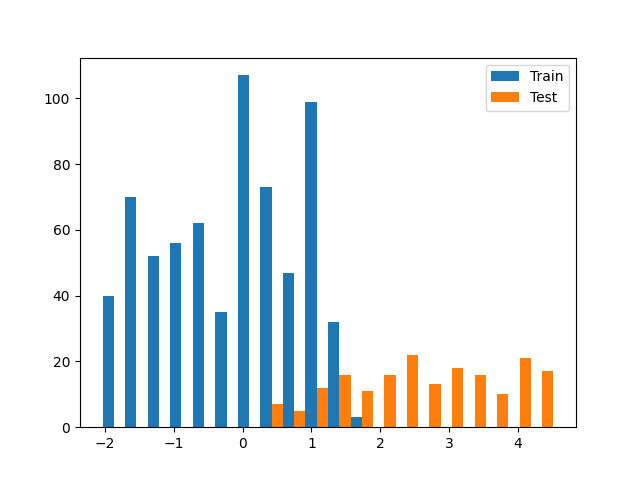
\includegraphics[scale=0.29]{img/ILI_channel6.png} 
		\end{minipage}
	}
\caption{Distribution of ETTh1, ETTh2, Electricity, and ILI dataset. A clear distribution shift between training and testing data can be observed in ETTh1, ETTh2, and ILI. } 
	\label{fig:distribution_shift} 
\end{figure*}


\begin{figure*}[h]	
	\subfigure[\textbf{24} steps-\textbf{ETTh1}]
	{
		\begin{minipage}{4.1cm}
			\centering     
			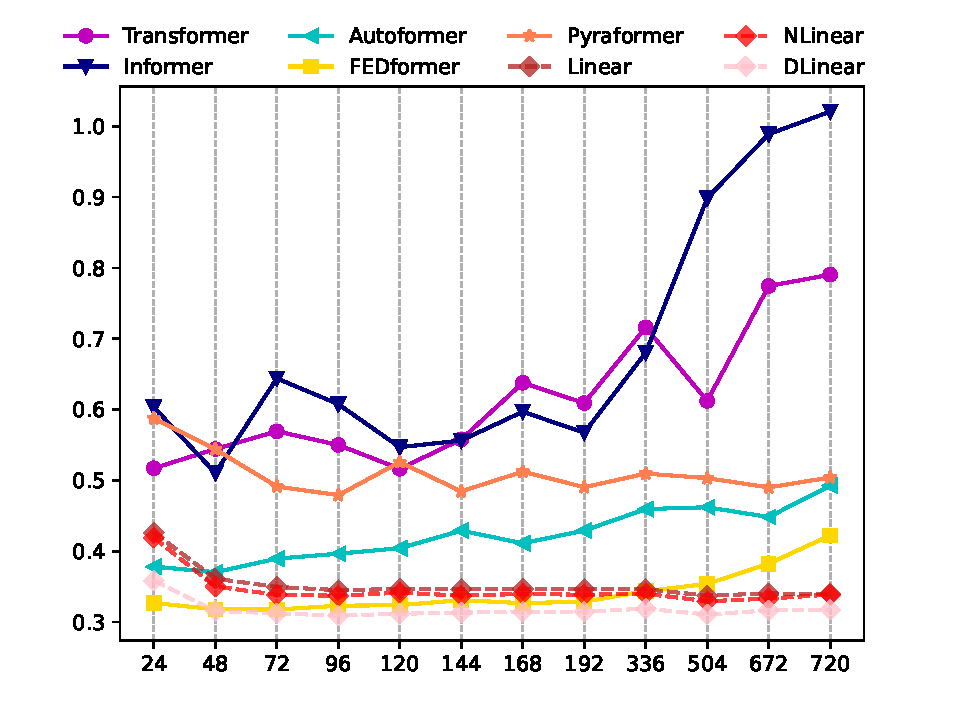
\includegraphics[scale=0.3]{img/Etth1_24.pdf}
		\end{minipage}
	}
	\subfigure[\textbf{720} steps-\textbf{ETTh1}]
	{
		\begin{minipage}{4.1cm}
			\centering     
			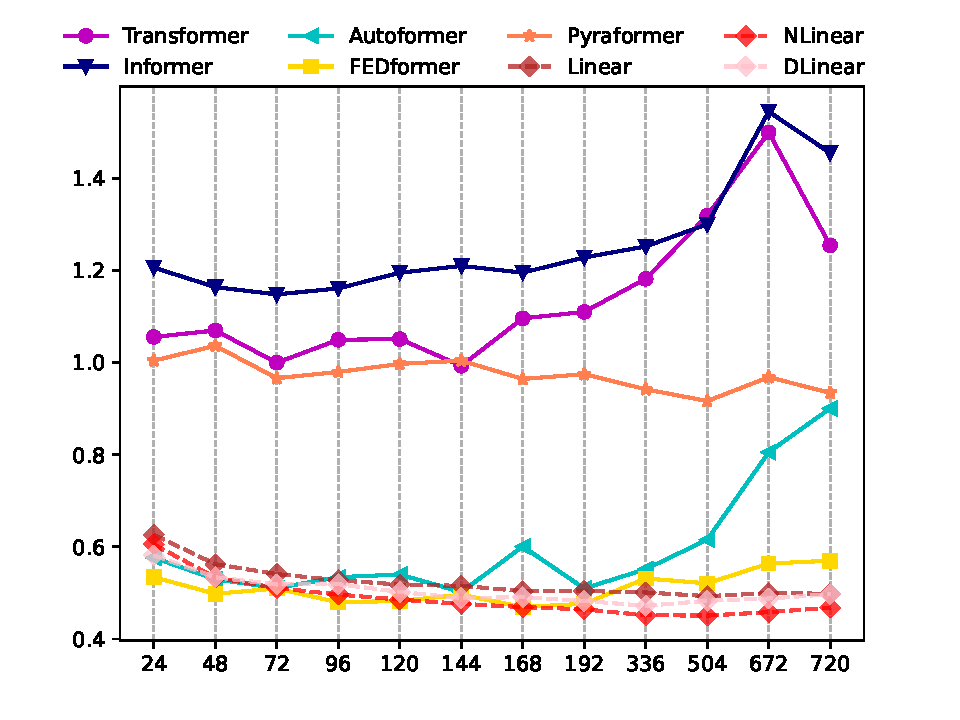
\includegraphics[scale=0.3]{img/Etth1_720.pdf} 
		\end{minipage}
	}
	\hspace{-2pt}
	\subfigure[\textbf{24} steps-\textbf{ETTh2}] 
	{
		\begin{minipage}{4.1cm}
			\centering         
			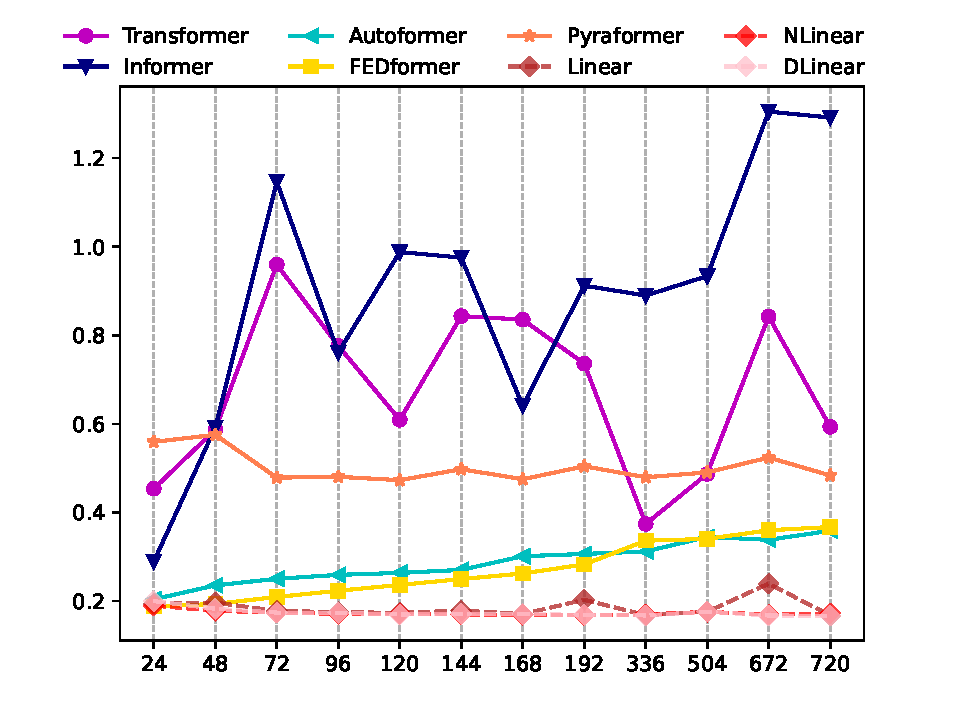
\includegraphics[scale=0.3]{img/Etth2_24.pdf} 
		\end{minipage}
	}
	\subfigure[\textbf{720} steps-\textbf{ETTh2}] 
	{
		\begin{minipage}{4.1cm}
			\centering      
			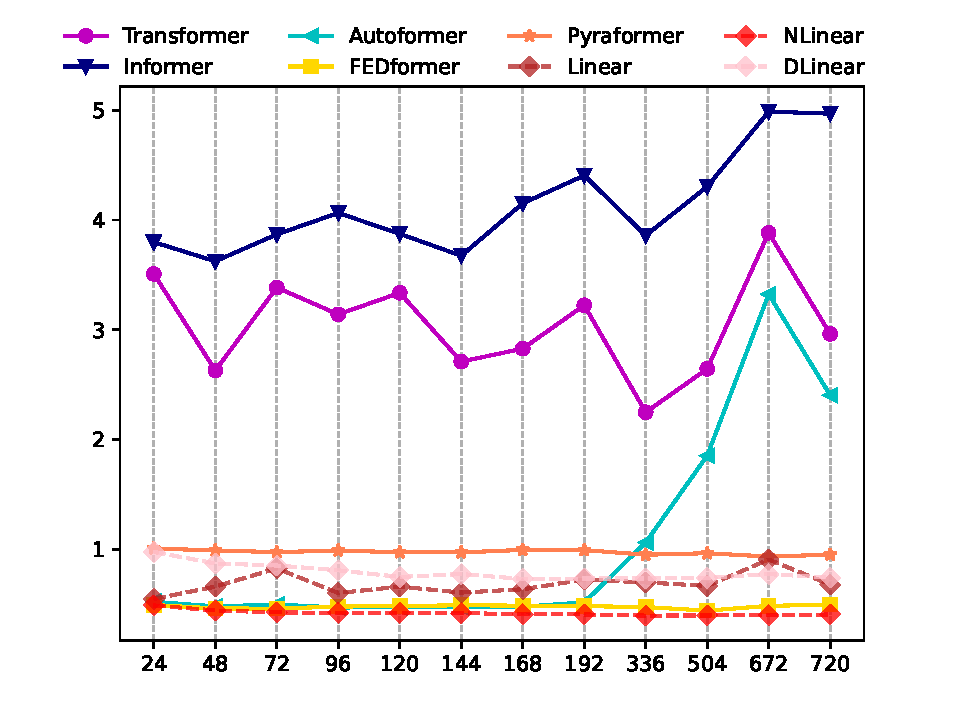
\includegraphics[scale=0.3]{img/Etth2_720.pdf}   
		\end{minipage}
	}
		\subfigure[\textbf{24} steps-\textbf{ETTm1}]
	{
		\begin{minipage}{4.1cm}
			\centering     
			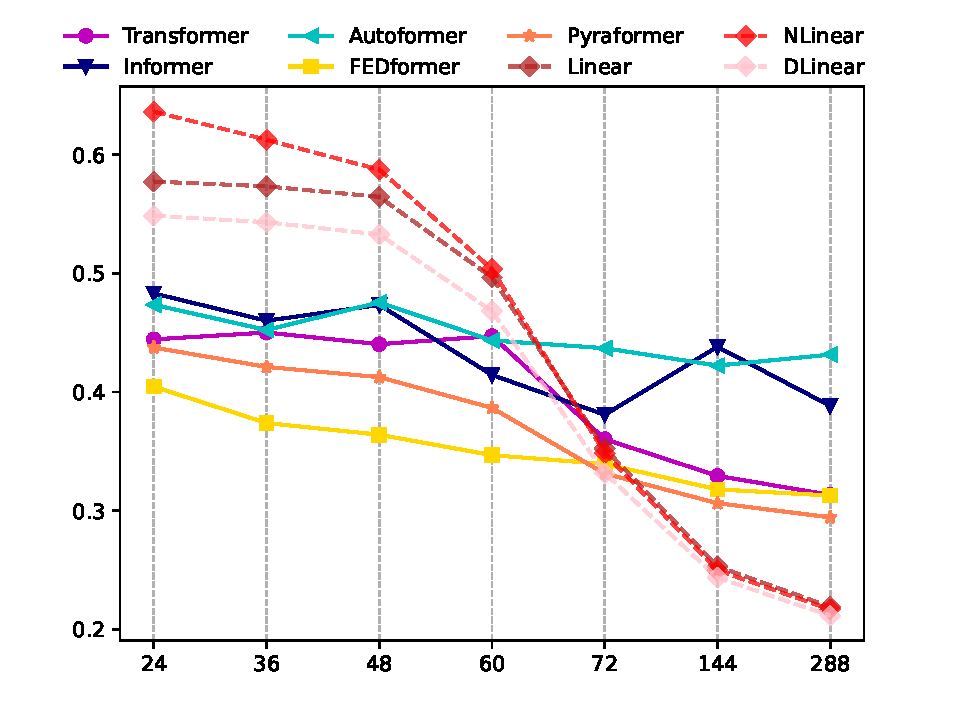
\includegraphics[scale=0.3]{img/Ettm1_24.pdf}
		\end{minipage}
	}
	\subfigure[\textbf{576} steps-\textbf{ETTm1}]
	{
		\begin{minipage}{4.1cm}
			\centering     
			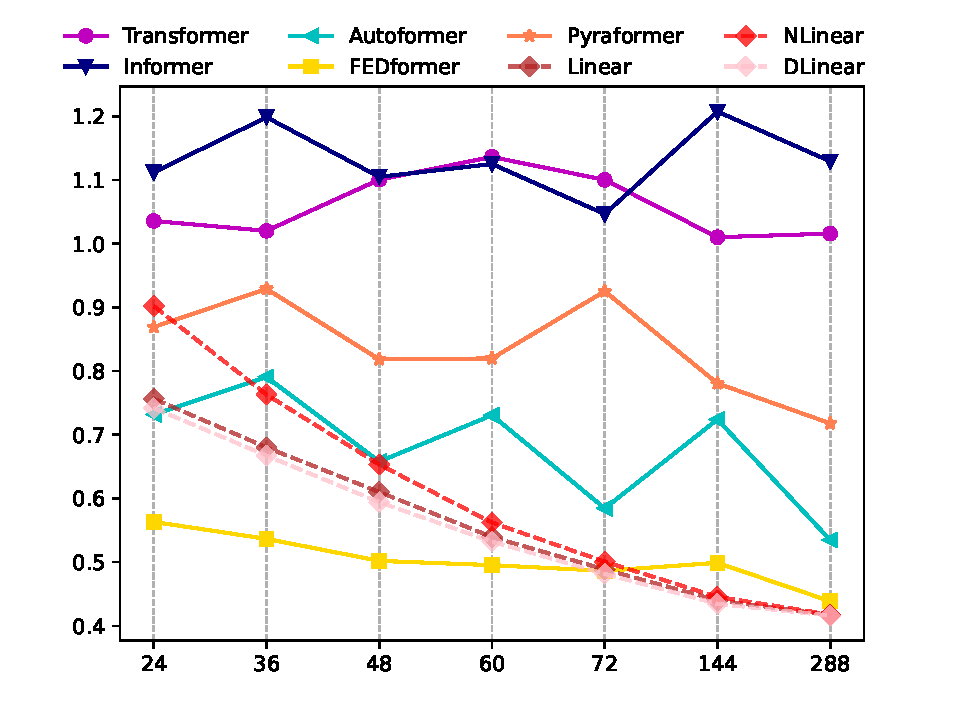
\includegraphics[scale=0.3]{img/Ettm1_576.pdf} 
		\end{minipage}
	}
	\hspace{-2pt}
	\subfigure[\textbf{24} steps-\textbf{ETTm2}] 
	{
		\begin{minipage}{4.1cm}
			\centering         
			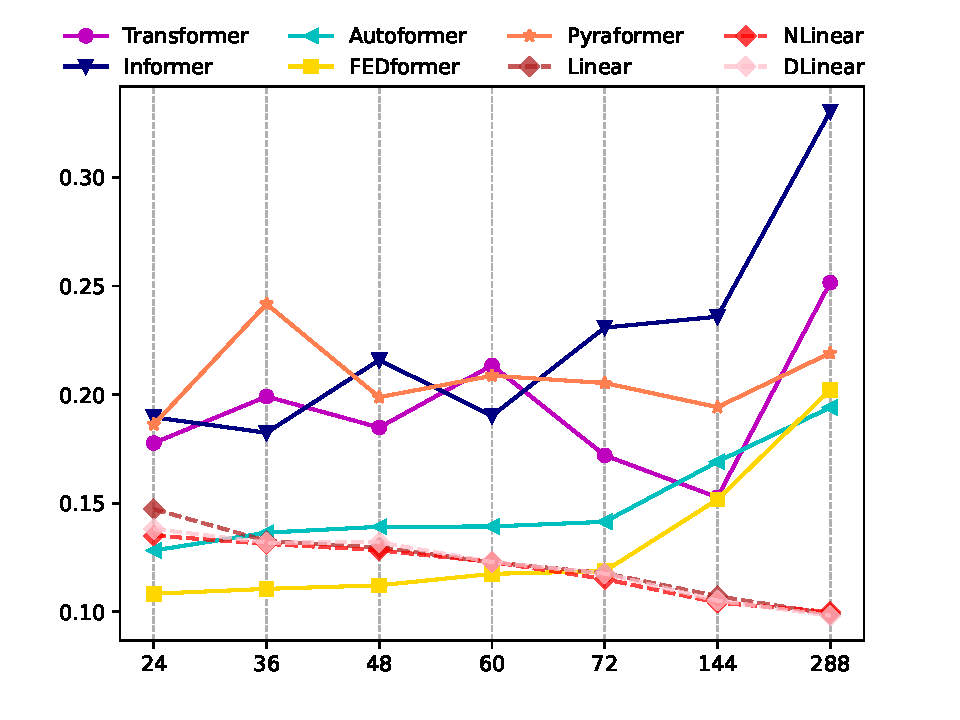
\includegraphics[scale=0.3]{img/Ettm2_24.pdf} 
		\end{minipage}
	}
	\subfigure[\textbf{576} steps-\textbf{ETTm2}] 
	{
		\begin{minipage}{4.1cm}
			\centering      
			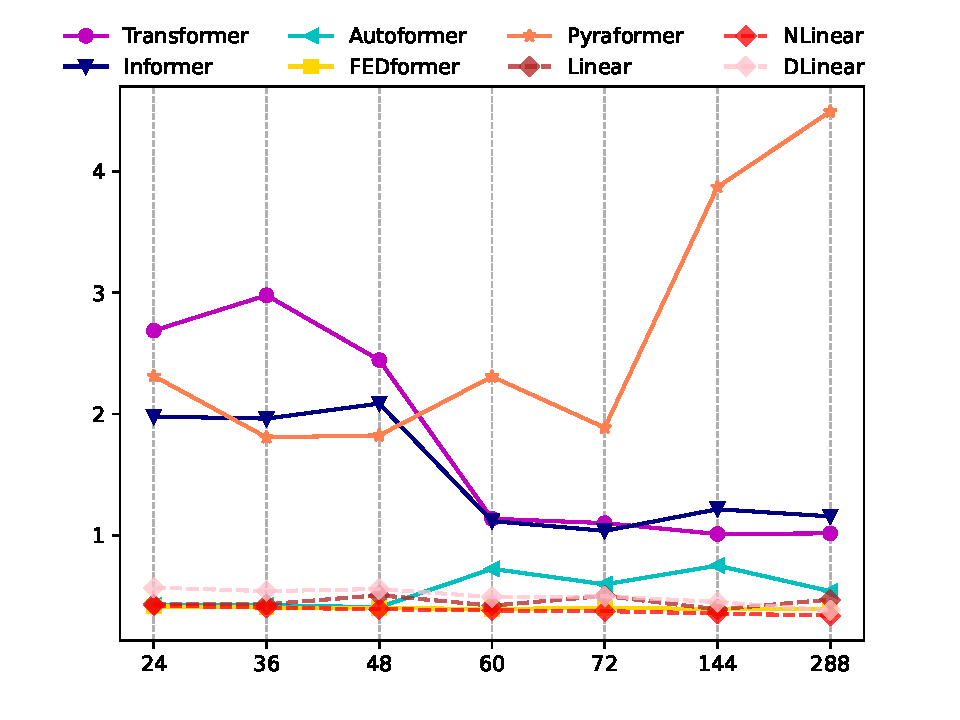
\includegraphics[scale=0.3]{img/Ettm2_576.pdf}   
		\end{minipage}
	}
	\subfigure[\textbf{24} steps-\textbf{Weather}] 
	{
		\begin{minipage}{4.1cm}
			\centering         
			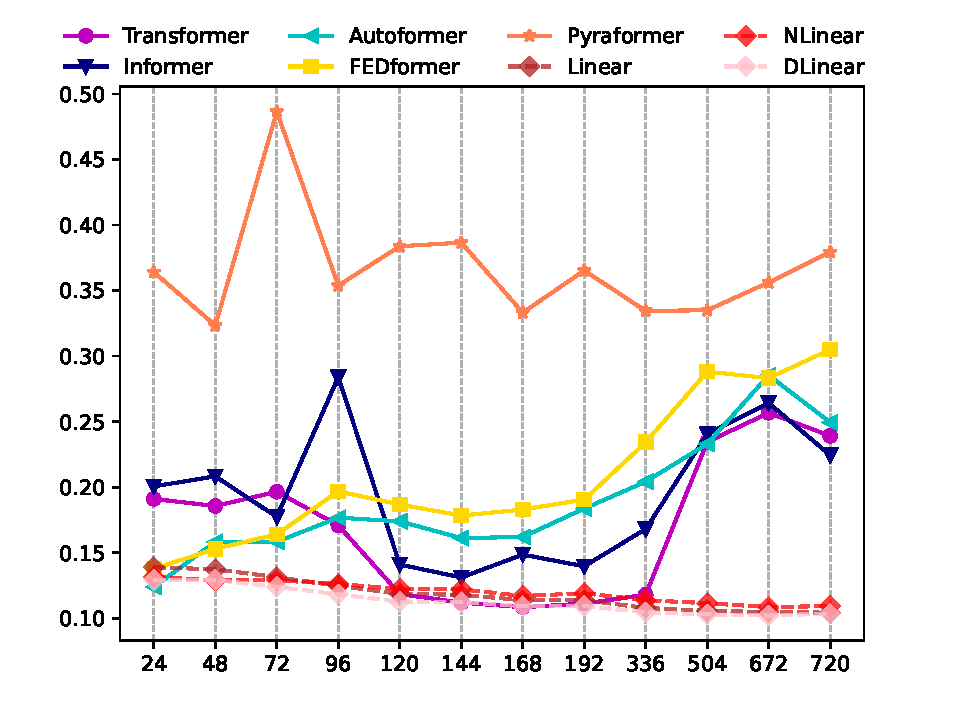
\includegraphics[scale=0.3]{img/weather_24.pdf} 
		\end{minipage}
	}
	\subfigure[\textbf{720} steps-\textbf{Weather}] 
	{
		\begin{minipage}{4.1cm}
			\centering      
			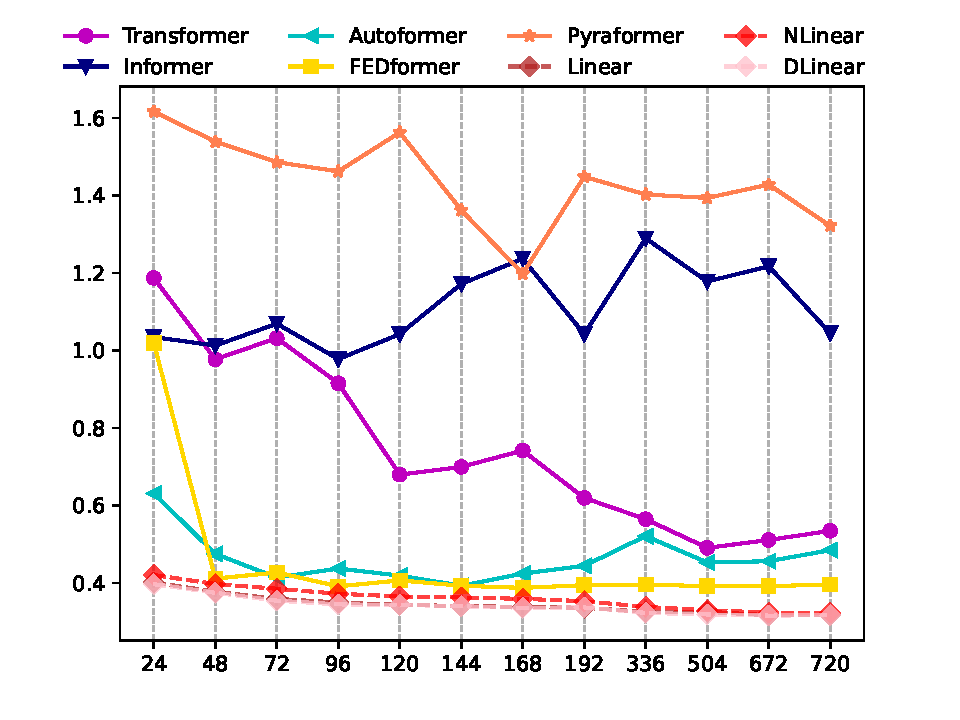
\includegraphics[scale=0.3]{img/weather_720.pdf}   
		\end{minipage}
	}
	\hspace{-2pt}
	\subfigure[\textbf{24} steps-\textbf{Traffic}]
	{
		\begin{minipage}{4.1cm}
			\centering     
			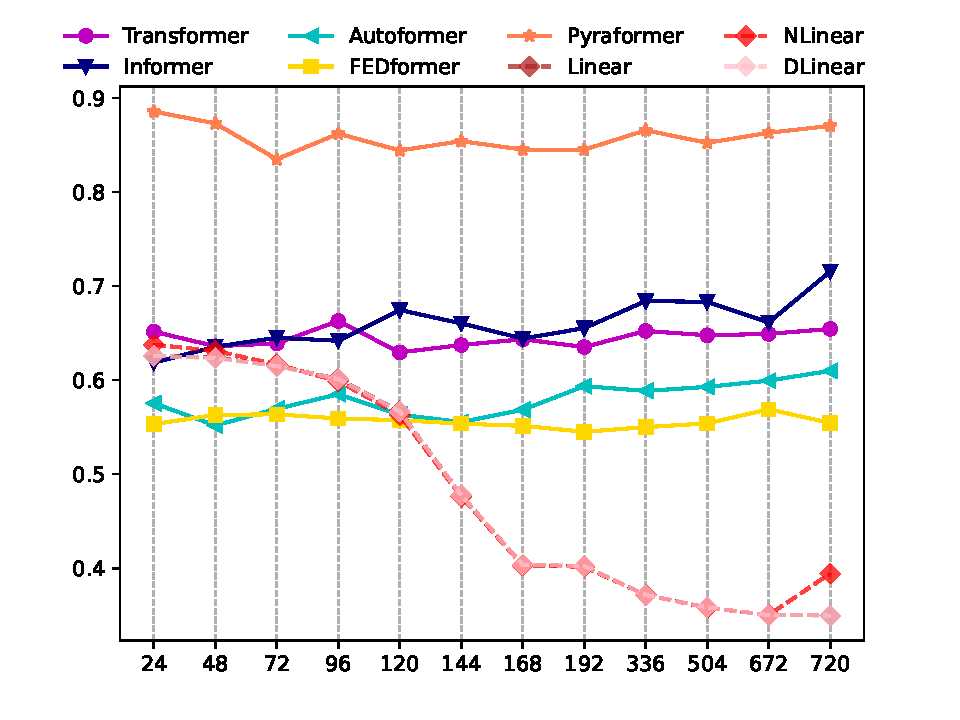
\includegraphics[scale=0.3]{img/traffic_24.pdf}
		\end{minipage}
	}
	\subfigure[\textbf{720} steps-\textbf{Traffic}]
	{
		\begin{minipage}{4.1cm}
			\centering     
			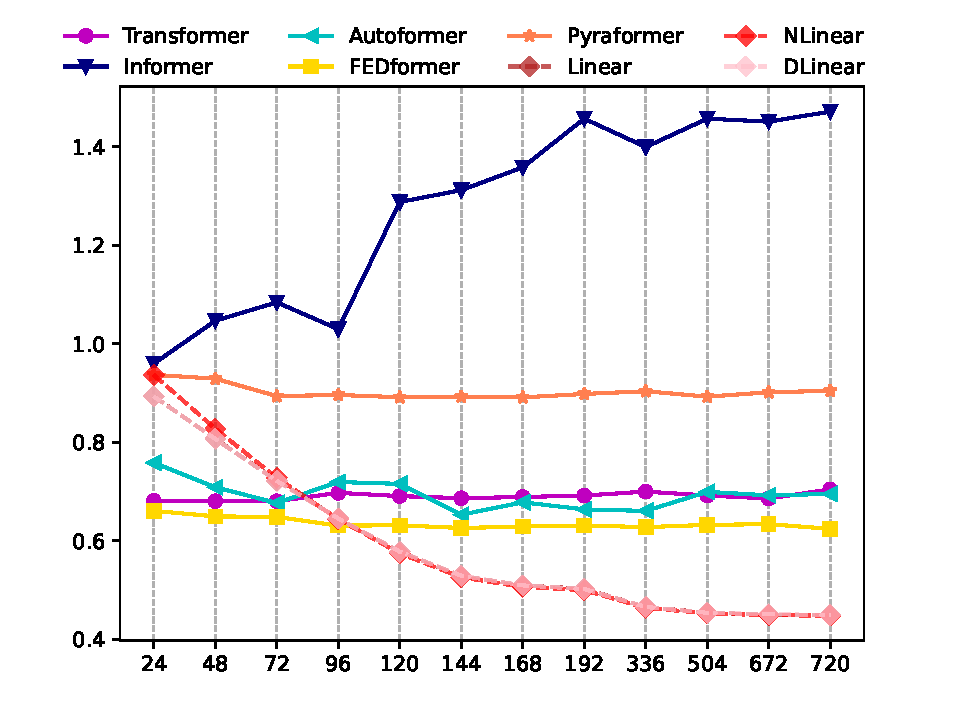
\includegraphics[scale=0.3]{img/traffic_720.pdf} 
		\end{minipage}
	}
	\subfigure[\textbf{24} steps-\textbf{Exchange}] 
	{
		\begin{minipage}{4.1cm}
			\centering         
			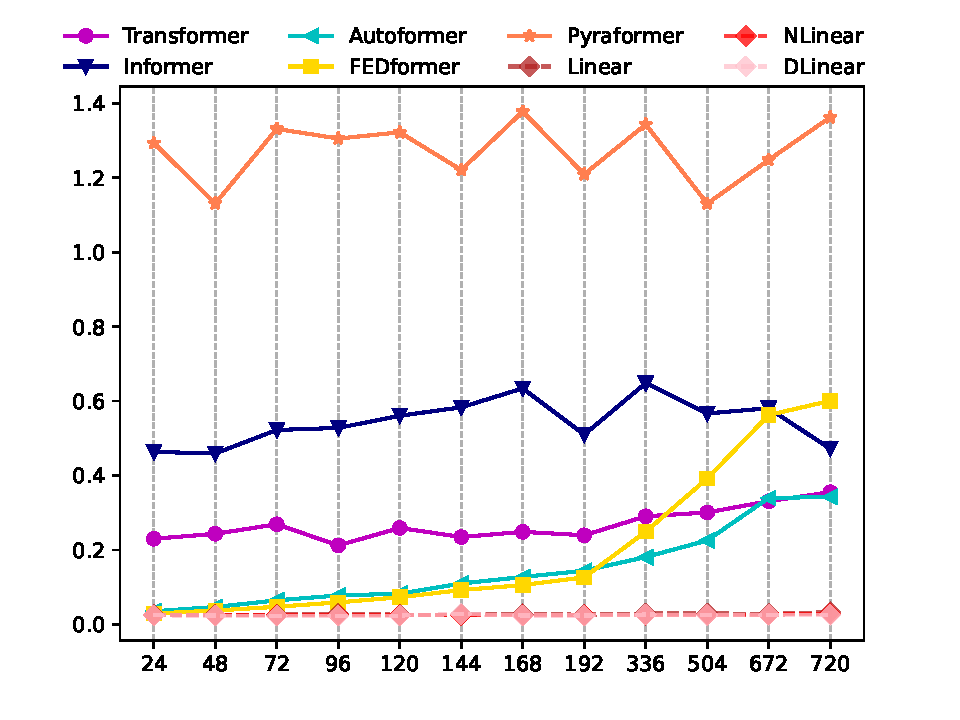
\includegraphics[scale=0.3]{img/exchange_rate_24.pdf} 
		\end{minipage}
	}
	\subfigure[\textbf{720} steps-\textbf{Exchange}] 
	{
		\begin{minipage}{4.1cm}
			\centering      
			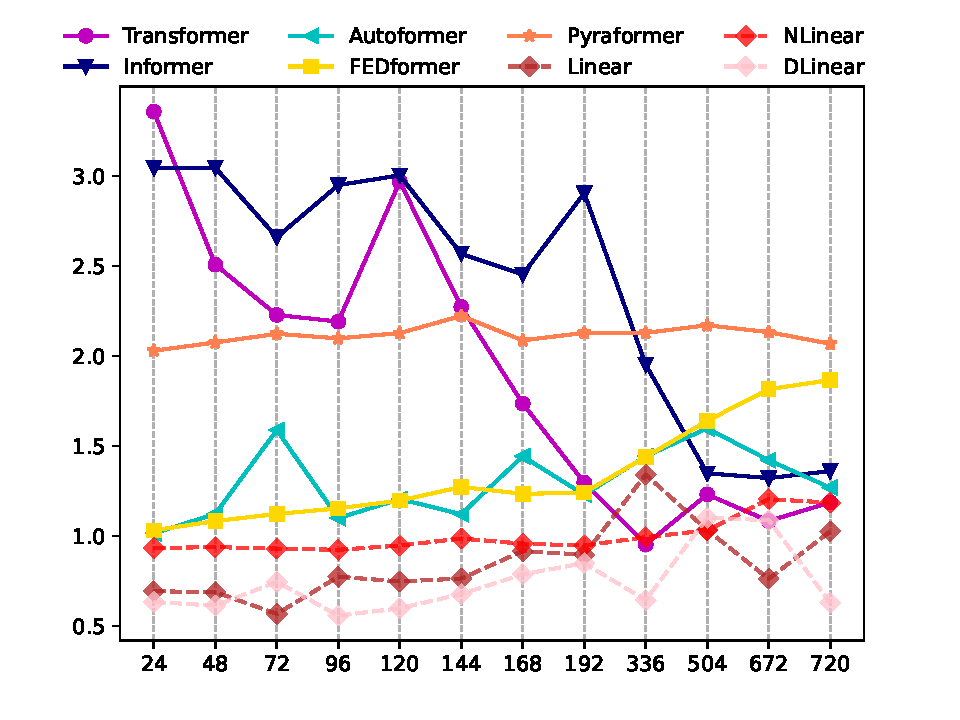
\includegraphics[scale=0.3]{img/exchange_rate_720.pdf}   
		\end{minipage}
	}
	\hspace{-2pt}
		\subfigure[\textbf{24} steps-\textbf{ILI}]
	{
		\begin{minipage}{4.1cm}
			\centering     
			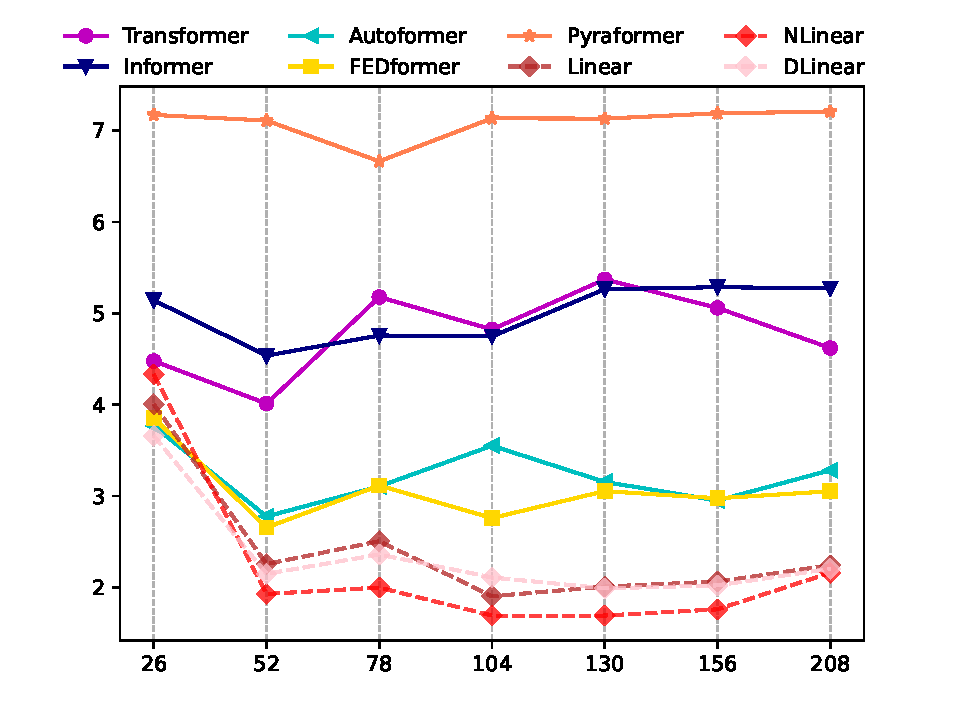
\includegraphics[scale=0.3]{img/ILI_24.pdf}
		\end{minipage}
	}
	\subfigure[\textbf{60} steps-\textbf{ILI}]
	{
		\begin{minipage}{4.1cm}
			\centering     
			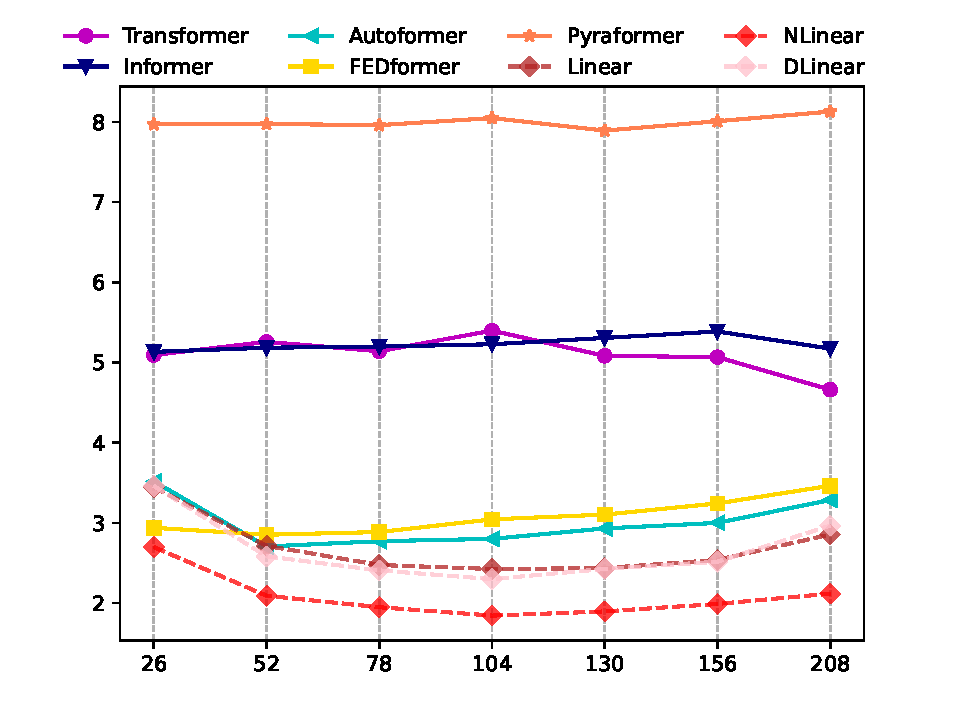
\includegraphics[scale=0.3]{img/ILI_60.pdf} 
		\end{minipage}
	}
	\caption{The MSE results (Y-axis) of models with different look-back window sizes (X-axis) of the long-term forecasting (e.g., \textbf{720}-time steps) and the short-term forecasting (e.g., \textbf{24} time steps) on different benchmarks. } 
	\label{fig:supp_lookBackWindows} 
\end{figure*}



\subsection{Comparison under Different Look-back Windows}

In Figure~\ref{fig:supp_lookBackWindows}, we provide the MSE comparisons of five LTSF-Transformers with \modelname under different look-back window sizes to explore whether existing Transformers can extract temporal well from longer input sequences. 
For hourly granularity datasets (ETTh1, ETTh2, Traffic, and Electricity), the increasing look-back window sizes are \{24, 48, 72, 96, 120, 144, 168, 192, 336, 504, 672, 720\}, which represent \{1, 2, 3, 4, 5, 6, 7, 8, 14, 21, 28, 30\} days. The forecasting steps are \{24, 720\}, which mean \{1, 30\} days. For 5-minute granularity datasets (ETTm1 and ETTm2), we set the look-back window size as \{24, 36, 48, 60, 72, 144, 288\}, which represent \{2, 3, 4, 5, 6, 12, 24\} hours. For 10-minute granularity datasets (Weather), we set the look-back window size as \{24, 48, 72, 96, 120, 144, 168, 192, 336, 504, 672, 720\}, which mean \{4, 8, 12, 16, 20, 24, 28, 32, 56, 84, 112, 120\} hours. The forecasting steps are \{24, 720\} that are \{4, 120\} hours. For weekly granularity dataset (ILI), we set the look-back window size as \{26, 52, 78, 104, 130, 156, 208\}, which represent \{0.5, 1, 1.5, 2, 2.5, 3, 3.5, 4\} years. The corresponding forecasting steps are \{26, 208\}, meaning \{0.5, 4\} years.

As shown in Figure~\ref{fig:supp_lookBackWindows}, with increased look-back window sizes, the performance of \modelname is significantly boosted for most datasets (e.g., ETTm1 and Traffic), while this is not the case for Transformer-based TSF solutions. Most of their performance fluctuates or gets worse as the input lengths increase. To be specific, the results of Exchange-Rate do not show improved results with a long look-back window (from Figure~\ref{fig:supp_lookBackWindows}(m) and (n)), and we attribute it to the low information-to-noise ratio in such financial data.


\begin{figure*}[h]
\begin{center}
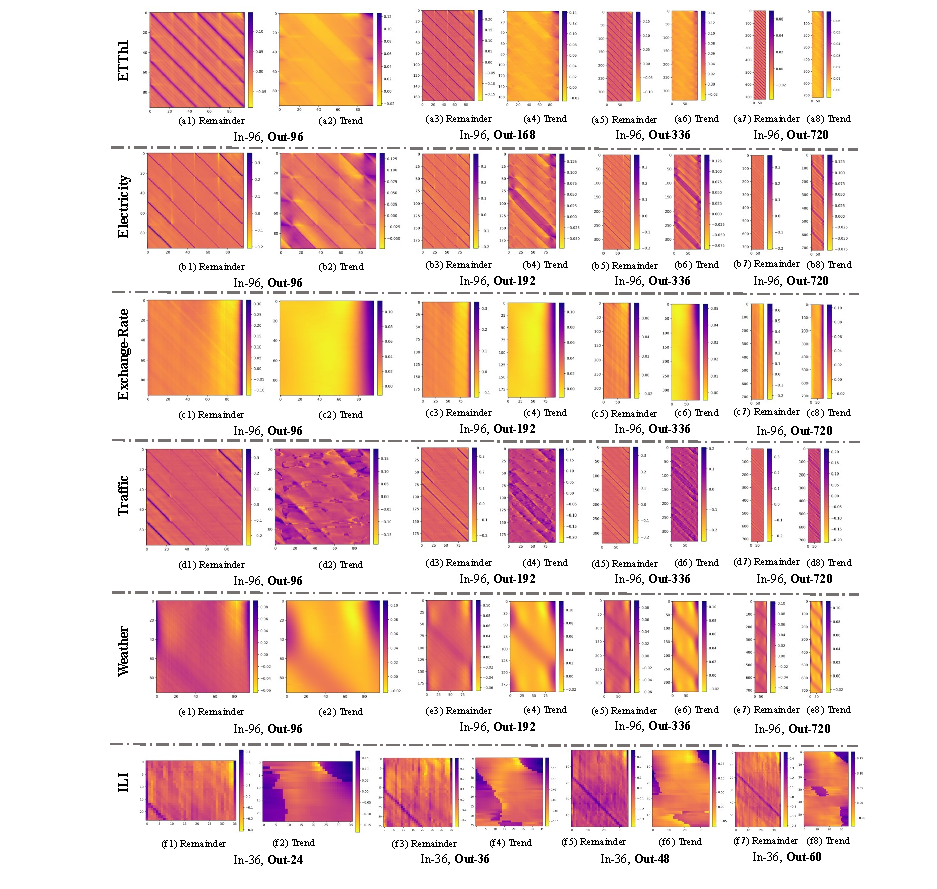
\includegraphics[width=1\textwidth]{img/viz.pdf}
\end{center}
\caption{Visualization of the weights(T*L) of \modelname on several benchmarks. Models are trained with a look-back window L (X-axis) and different forecasting time steps T (Y-axis). We show weights in the remainder and trend layer.}
\label{fig:viz}
\end{figure*}

\section{Ablation study on the \modelname}
\label{sec:supp_lookback}



\subsection{Motivation of NLinear}
% 
If we normalize the test data by the mean and variance of train data, there could be a distribution shift in testing data, i.e, the mean value of testing data is not 0. If the model made a prediction that is out of the distribution of true value, a large error would occur. For example, there is a large error between the true value and the true value minus/add one. Therefore, in \emph{NLinear}, we use the subtraction and addition to shift the model prediction toward the distribution of true value. Then, large errors are avoided, and the model performances can be improved.
%
Figure~\ref{fig:distribution_shift} illustrates histograms of the trainset-test set distributions, where each bar represents the number of data points. Clear distribution shifts between training and testing data can be observed in ETTh1, ETTh2, and ILI. Accordingly, from Table~\ref{tab:uni-benchmarks-ett} and Table 2 in the main paper, we can observe that there are great improvements in the three datasets comparing the \emph{NLinear} to the \emph{Linear}, showing the effectiveness of the \emph{NLinear} in relieving distribution shifts. Moreover, for the datasets without obvious distribution shifts, like Electricity in Figure~\ref{fig:distribution_shift}(c), using the vanilla \emph{Linear} can be enough, demonstrating the similar performance with \emph{NLinear} and \emph{DLinear}.






\subsection{The Features of LTSF-Linear}


Although \modelname is simple, it has some compelling characteristics:

\begin{itemize}
\item \textbf{An $O(1)$ maximum signal traversing path length}: The shorter the path, the better the dependencies are captured~\cite{liu2021pyraformer}, making \modelname capable of capturing both short-range and long-range temporal relations.


\item \textbf{High-efficiency:} As \modelname is a linear model with two linear layers at most, it costs much lower memory and fewer parameters and has a faster inference speed than existing Transformers (see Table $8$ in main paper). 



\item \textbf{Interpretability:} After training, we can visualize weights from the seasonality and trend branches to have some insights on the predicted values~\cite{dong2008granular}. 


\item \textbf{Easy-to-use:} \modelname can be obtained easily without tuning model hyper-parameters.


\end{itemize}

\subsection{Interpretability of LTSF-Linear} 
Because \modelname is a set of linear models, the weights of linear layers can directly reveal how \modelname works. The weight visualization of \modelname can also reveal certain characteristics in the data used for forecasting.

Here we take DLinear as an example. Accordingly, we visualize the trend and remainder weights of all datasets with a fixed input length of 96 and four different forecasting horizons. To obtain a smooth weight with a clear pattern in visualization, we initialize the weights of the linear layers in DLinear as $1/L$ rather than random initialization. That is, we use the same weight for every forecasting time step in the look-back window at the start of training. 

\textbf{How the model works:} Figure~\ref{fig:viz}(c) visualize the weights of the trend and the remaining layers on the Exchange-Rate dataset. Due to the lack of periodicity and seasonality in financial data, it is hard to observe clear patterns, but the trend layer reveals greater weights of information closer to the outputs, representing their larger contributions to the predicted values.

\textbf{Periodicity of data:} For Traffic data, as shown in Figure~\ref{fig:viz}(d), the model gives high weights to the latest time step of the look-back window for the {0,23,47...719} forecasting steps. Among these forecasting time steps, the {0, 167, 335, 503, 671} time steps have higher weights. Note that 24 time steps are a day, and 168 time steps are a week. This indicates that Traffic has a daily periodicity and a weekly periodicity.

